\documentclass{standalone}
\usepackage{tikz}
\usepackage{ctex,siunitx,ninecolors}
\setCJKmainfont{Noto Serif CJK SC}
\usepackage{tkz-euclide}
\usepackage{amsmath}
\usetikzlibrary{patterns, calc}
\usetikzlibrary {decorations.pathmorphing, decorations.pathreplacing, decorations.shapes}
\begin{document}
\small
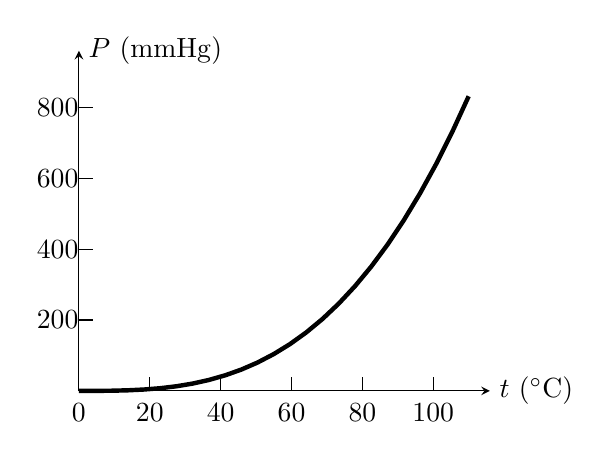
\begin{tikzpicture}[>=stealth, scale=0.9,domain=0:5.5]
  % \useasboundingbox(-1.4,-1.4)rectangle(1.4,1.4);
  \draw[<->] (0,4.8)node [right]{$P$ (\unit{mmHg})}--(0,0)--(5.8,0)node [right]{$t$ (\unit{\celsius})};
  \foreach \x in{1,2,3,4}
  {
     \draw(0,\x)--(.2, \x);
  }
  \foreach \x in{1,2,3,4,5}
  {
     \draw(\x,0)--(\x, .2);
  }
  \node at (-.3,1){200};\node at (-.3,2){400};\node at (-.3,3){600};\node at (-.3,4){800};
  \node at (1,-.3){20};\node at (2,-.3){40};\node at (3,-.3){60};\node at (4,-.3){80};\node at (5,-.3){100};\node at (0,-.3){0};
  \draw[color=black, ultra thick] plot (\x,{0.025*\x*\x*\x}) ;
\end{tikzpicture}
\end{document}